\section{Overview of Plasma Physics}
A \emph{plasma} is a quasi-neutral gas of ions, electrons, and neutral particles, which exhibit collective behavior. Plasmas can behave in similar ways to a conventional fluid -- they can flow, they can be compressible, they can be turbulent, and so on -- however the addition of charged particles facilitates many behaviors unique to a plasma. Charged particles can interact with each other not just through ballistic collisions, but at a distance through electromagnetic forces. The bulk motion of a plasma can be manipulated through electric and magnetic fields; conversely a plasma can have a substantial effect on the propagation of radio waves passing through it. 

A plasma can be analyzed in several different domains: Single particle motion; fluid approximations; and full kinematic solutions. In this work we treat the motions of electrons in the single particle domain, which is a natural choice for the sparse densities and small gyroradii of radiation belt electrons. To understand the behavior of radio waves propagating through a plasma, we treat the background as a smooth dielectric medium. 

\subsection{Single Particle Motion}
The high energies and sparse densities of the radiation belts lend themselves very well to a single-particle approximation. Many of the basic behaviors and quantities in plasma physics can be understood through studying the motion of a single particle.

The fundamental equation of motion for a charged particle in an electromagnetic field is given by the Lorentz force:
\begin{equation}
\vec{F} = \frac{d\vec{p}}{d\emph{t}} = q(\vec{E} + \vec{v}\times\vec{B})
\label{eqn:lorentz_force}
\end{equation}
Where $q$ represents the particle's charge, $\vec{E}$ and $\vec{B}$ represent the electric and magnetic fields, and $\vec{v}$ the particle's velocity, shown here in a non-relativistic frame.

Electric fields simply apply a force in the direction of the field. However, note that a cross product is perpendicular to both terms -- therefore any forces induced by the magnetic field will be perpendicular to the particle's velocity. The magnetic field is a \emph{conservative} force, in that a stationary magnetic field cannot directly impart energy into a particle, but can alter a particle's trajectory. The particle will therefore have a net drift in the direction of the electric field, while exhibiting a helical motion around the magnetic field.

We can then split the velocity vector into two quantities -- $v_\parallel$ parallel to the magnetic field, and $v_\perp$ perpendicular to the magnetic field.

Two characteristic values arise from this motion: the radius of the particle's rotation around the magnetic field, known as the \emph{gyroradius} or the \emph{Larmor radius}:
\begin{equation}
r_l = \frac{m v_\perp}{qB}
\end{equation}

And the rotation frequency, known as the \emph{gyrofrequency} or \emph{cyclotron frequency}:
\begin{equation}
\omega_c = \frac{v_\perp}{r_l} = \frac{q B}{m} \quad \unit{rad/sec}
\end{equation}

By integrating the particle's momentum over a single gyrorotation, we arrive at a third fundamental quantity known as the magnetic moment, or the \emph{first adiabatic invariant}:
\begin{equation}
\mu = \frac{m v_\perp^2}{2B}
\label{eqn:mu}
\end{equation}

In situations where the magnetic field varies slowly (e.g., on spatial scales much greater than the gyroradius), then $\mu$ remains a constant of motion.

A final parameter to describe a particle's motion is it's \emph{pitch angle}, the angle between the velocities perpendicular and parallel to the magnetic field:
\begin{equation}
\alpha = \mathrm{tan}^{-1}\bigg(\frac{v_\perp}{v_\parallel}\bigg)
\end{equation}

The first adiabatic invariant describes an implicit relationship between the magnetic field strength and a particle's pitch angle at a given point. 
Combining the first adiabatic invariant with conservation of kinetic energy, we can deduce an expression for magnetic trapping -- that is, the magnetic field strength in which a particle exhibiting helical motion along a magnetic field line will turn around at. 
\begin{eqnarray}
& E &= \frac{1}{2}mv^2 \\
& &= \frac{1}{2}m(v_\parallel^2 + v_\perp^2) \\
 & &= \frac{1}{2}mv^2(\mathrm{cos}^2\alpha + \mathrm{sin}^2\alpha)
\end{eqnarray}

At a reflection point, the particle's kinetic energy will be entirely in the perpendicular mode:
\begin{eqnarray}
\frac{v_{\perp0}^2}{B_0} = \frac{v_{\perp1}^2}{B_1} \\
\frac{v^2\mathrm{sin}^2(\alpha)}{B_0} = \frac{v^2}{B_1} \\
\mathrm{sin}^2(\alpha)=\frac{B_0}{B_1} 
\end{eqnarray}

Therefore, a charged particle in a magnetic field will be constrained to rotate around a field line, and bounce back and forth, reflecting where the magnetic field strength increases. A key takeaway is that the reflection point is independent of energy, and depends only on the ratio of magnetic field strengths and the particle's initial pitch angle. An example of this behavior is shown in figure \ref{fig:bottle}.
\begin{figure}[ht]
\begin{center}
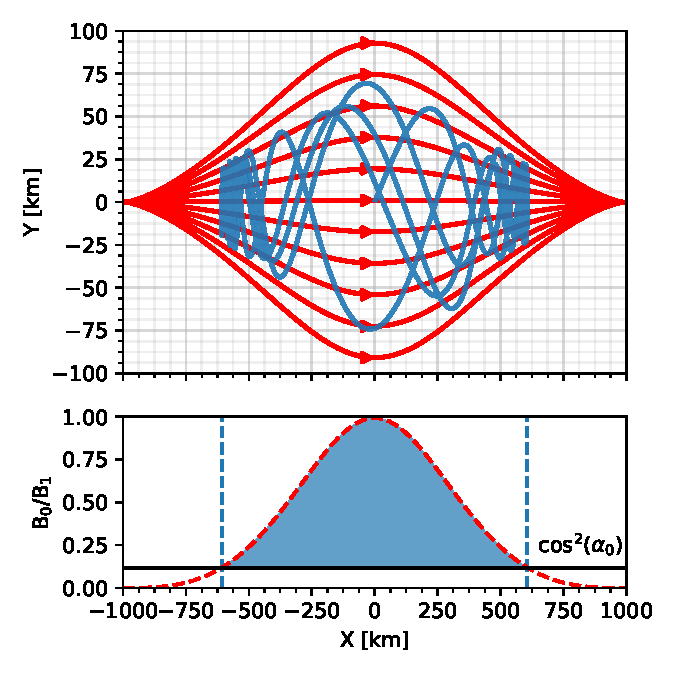
\includegraphics{figures/bottle.pdf}
\caption{An example of a ``magnetic bottle" particle trap. The top plot shows the trajectory of an electron with an initial pitch angle $\alpha_0=20^\circ$. The bottom plot shows the magnetic field ratio $B_0/B_1$, with the particle's reflection points shown as vertical lines. }
\label{fig:bottle}
\end{center}
\end{figure}










\subsection{Waves in Plasmas}
Previously, we have described the motion of a charged particle under the influence of an electromagnetic field. the single-particle approximation provides enormous insight into the dynamics of a sparsely-populated plasma. Next, we must consider the inverse system -- how the charged particles in a plasma dictate the characteristic behaviors of an electromagnetic wave propagating through it.

An electromagnetic wave can accelerate a charged particle; conversely, an accelerating or decelerating particle induces its own electromagnetic field. It would seem, then, that the behavior of an electromagnetic field in a plasma is simply the summation of the contributions of each particle. However, the complexity of this brute-force approach quickly becomes intractable for even a handful of particles. The universal approach taken then is to abstract the complicated interplay of waves and particles into a wave moving through a dielectric medium, described only by the various constituent densities, temperatures, and background field intensities within a given volume. 

As with any electromagnetic problem, we begin with Maxwell's equations -- shown here in their non-relativistic, differential form, in SI units:

\begin{eqnarray}
&\nabla \cdot \vec{E}& = \frac{\rho}{\epsilon_0} \label{eqn:maxwell1}\\
&\nabla \cdot \vec{B}& = 0 \label{eqn:maxwell2}\\
&\nabla \times \vec{E}& = -\frac{\partial \vec{B}}{\partial t} \label{eqn:maxwell3}\\
&\nabla \times \vec{B}& = \mu_0 \vec{J} + \frac{1}{c^2}\frac{\partial \vec{E}}{\partial t} \label{eqn:maxwell4}
\end{eqnarray}

$\vec{E}$ and $\vec{B}$ denote the electric and magnetic fields; $\mu_0$ and $\epsilon_0$ denote the magnetic permeability and electric permittivity of free space; and $c=\sqrt{\frac{1}{\mu_0\epsilon_0}}$ is the speed of light. The terms $\rho$ and $\vec{J}$ represent the local charge density and current density, both of which are a function of position and time.

By taking the curl of equation \ref{eqn:maxwell3} and substituting in the time derivative of equation \ref{eqn:maxwell4}, and making use of the vector identity $\nabla \times \nabla \times \vec{E} = \nabla(\nabla \cdot \vec{E}) - \nabla^2\vec{E}$, we have:

\begin{equation}
\nabla^2\vec{E} - \frac{\nabla\rho}{\epsilon_0} = \mu_0 \frac{\partial \vec{J}}{\partial t} + \frac{1}{c^2}\frac{\partial^2\vec{E}}{\partial t^2}
\label{eqn:dielectric_tensor_derivation_1}
\end{equation}

In the absence of charges or currents ($\rho=0$, $\vec{J}=0$), the equation reduces to the free-space wave equation:
\begin{equation}
\nabla^2\vec{E} = \frac{1}{c^2}\frac{\partial^2\vec{E}}{\partial t^2}
\end{equation}

Next, we linearize the system and search for harmonic perturbations of the form:
\begin{eqnarray}
\vec{E(\vec{r},t)} = \vec{E_1}e^{{i (\omega t - \vec{k}\cdot \vec{r}})} \label{eqn:linear1}\\ 
\vec{B(\vec{r},t)} = \vec{B_0} + \vec{B_1}e^{{i (\omega t - \vec{k}\cdot \vec{r}})} \label{eqn:linear2}\\
\vec{J(\vec{r},t)} = \vec{J_1}e^{{i (\omega t - \vec{k}\cdot \vec{r}})}\label{eqn:linear3} 
\end{eqnarray}

where $\omega$ is the wave angular frequency, $\vec{k}$ is the wave vector, or spatial frequency, and $\vec{r}$ is the spatial coordinate. Two fundamental parameters of an electromagnetic wave are the \emph{phase velocity}, $\omega/k$, and the \emph{group velocity}, $\partial\omega/\partial k$. The relation between the temporal and spatial frequencies is known as the \emph{dispersion relation}.

From here we follow the derivation and convention used by \cite{Stix1992}. In general, a plasma is comprised of several different species of constituent particles -- positively and negatively charged particles necessary to maintain a quasi-neutral plasma. While the dispersion relations of different species cannot be simply added, their effects can be summed to form the displacement current $\vec{J}$:
\begin{equation}
\vec{J} = \sum_s\vec{J_s} = \sum_s n_s q_s \vec{u_s}
\label{eqn:J}
\end{equation}
where $n$, $q$, and $\vec{u}$ represent the density, charge, and velocity of a particular species $s$. 

We make the assumption that the plasma is \emph{cold} -- that is, that the velocities of each species $\vec{u_s}$ have a single value each. Were we to relax this assumption, each species density would have a distribution function in both position and momentum, $n=n(\vec{r},\vec{p})$. For a treatment of a hot plasma, see the work by \cite{Sazhin1993}.

Next, we note that, in a cold plasma assumption, the Lorentz force (equation \ref{eqn:lorentz_force}) can be written for each species:
\begin{equation}
m_s\frac{d\vec{u_s}}{dt} = q_s\big(\vec{E} + \vec{u_s}\times\vec{B}\big) 
\label{eqn:lorentz_2}
\end{equation}
Combining equations \ref{eqn:linear1} -- \ref{eqn:linear3}, \ref{eqn:J}, and \ref{eqn:lorentz_2}, and assuming a coordinate system with the background magnetic field $\vec{B_0}$ aligned with the z-axis, we arrive at an expression for the \emph{cold-plasma dielectric tensor}:

\begin{equation}
\vec{\epsilon}\cdot\vec{E}=\begin{pmatrix}
S & -iD & 0 \\
iD & S & 0 \\
0 & 0 & P \end{pmatrix}\begin{pmatrix}E_x \\ E_y \\ E_z\end{pmatrix}
\end{equation}

The various summations over each constituent species are incorporated into the so-called Stix parameters (\cite{Stix1992}):
\begin{eqnarray}
S =\frac{1}{2}(R + L) \qquad D = \frac{1}{2}(R - L)
\end{eqnarray}
\begin{equation}
R = 1 - \sum_s\frac{\omega_{ps}^2}{\omega(\omega + \omega_{Hs})}; \quad L = 1 - \sum_s\frac{\omega_{ps}^2}{\omega(\omega - \omega_{Hs})}; \quad P = 1 - \sum_s\frac{\omega_{ps}^2}{\omega^2}
\end{equation}

where $\omega_{ps} = n_sq_s^2/{\epsilon_0 m_s}$ and $\omega_{Hs}=q_sB_0/m_s$ are the plasma and cyclotron frequencies for species $s$.

\subsubsection{Dispersion Relation}
With the dielectric tensor now determined, we can derive the relationship between $\omega$ and $\vec{k}$, known as the dispersion relation. Equation \ref{eqn:dielectric_tensor_derivation_1} can be written as:
\begin{equation}
\vec{\mu}\times \vec{\mu} \times \vec{E} +  \epsilon\cdot\vec{E} = 0
\end{equation}
where $\mu = \vec{k}c/\omega$ is the wave refractive index. Assuming a wave propagating with some angle $\theta$ between $\vec{mu}$ and the background magnetic field, we arrive at:
\begin{equation}
\begin{pmatrix}
S - \mu^2\cos^2\theta & -iD & \mu^2\cos{\theta}\sin{\theta} \\
iD & S - \mu^2 & 0 \\
\mu^2\cos{\theta}\sin{\theta} & 0 & P - \mu^2\sin^2{\theta} \end{pmatrix}\begin{pmatrix}E_x \\ E_y \\ E_z\end{pmatrix} = 0
\label{eqn:dispersion_relation_matrix}
\end{equation}

Taking the determinant of \ref{eqn:dispersion_relation_matrix} yields the \emph{cold-plasma dispersion relation}:

\begin{eqnarray}
&A\mu^4 - B\mu^2 + C &= 0 \label{eqn:disp_rln}  \\
&A& = S \sin^2\theta + P\cos^2\theta \\
&B& = RL\sin^2\theta + PS(1 + \cos^2\theta) \\
&C& = PRL
\end{eqnarray}

We can solve for $\mu^2 = k^2c^2/\omega^2$ using the quadratic formula.

Finally, it is worth noting that when considering a single-species plasma (e.g., electrons only), equation \ref{eqn:disp_rln} reduces to the \emph{Appleton-Hartree Equation} (\cite{Appleton1932}):


\begin{equation}
\mu^2 = 1 - \frac{\frac{\omega_{pe}^2}{\omega^2}}{1 - \frac{\omega_{He}^2\sin^2\theta}{2(\omega^2 - \omega_{pe}^2)} \pm\big[\big(\frac{\omega_{He}^2\sin^2\theta}{2(\omega^2 - \omega_{pe}^2)}\big)^2 + \frac{\omega_{He}^2}{\omega^2}\cos^2\theta\big]^{1/2}}
\end{equation}
For a simpler derivation of the Appleton-Hartree equation alone, see the classic, approachable text by \cite{Chen1983}.

The dispersion relation in equation \ref{eqn:disp_rln} reveals a wealth of information about the characteristics of waves in plasmas. For various plasma densities and background magnetic field strength, we can infer which wave frequencies may propagate, if any, and which wave polarizations. Through the remainder of this work, we will be concerned with the \emph{Whistler} mode -- a right-hand, circularly-polarized (RHCP) wave. Within a typical magnetospheric plasma, the Whistler mode spans the VLF band, roughly between 30 Hz and 300 kHz.
\section{Coordinate Systems}
\section{Lightning Illumination Model}


\subsection{Emission Spectrum}
While a terrestrial lightning flash consists of several repeated strokes at varying incident angles, we adopt the simplified model used by \citealt{Lauben1998}, \citealt{Bortnik2005}, and subsequent workers.

The lightning flash is modeled as a single, vertical current pulse from a height $H_E$, with a time profile given by equation \ref{eqn:td_pulse}:
\begin{equation}
\label{eqn:td_pulse}
I(t)=I_0(e^{-a t} - e^{-b t})
\end{equation}

We relate the time-domain current profile to radiated power using the far-field approximation for an arbitrary source, given by \cite{Griffiths1999}, page 457:
\begin{equation}
\label{eqn:griffiths_power}
S(t) \approx \frac{1}{\mu_0}(\mathbf{E} \times \mathbf{B}) = \frac{\mu_0}{16\pi^2c}\left[\ddot{p}(t)\right]^2 \left(\frac{\sin^2\theta}{r^2}\right)\mathbf{\hat{r}}
\end{equation}

where $p(t)$ is the dipole moment given by $p=2 H_E \int_0^t{I(t)}dt$, r is the distance from the flash in meters, and $\theta$ is the angle to the flash. Taking the second derivative of the dipole moment (the first derivative of the current profile) gives us the far-field time-domain power equation:

\begin{equation}
\label{eqn:farfield_power_td}
S(t) = \frac{1}{Z_0}\left(\frac{\mu_0 H_E I_0}{2 \pi}\right)^2\left(\frac{\sin^2\theta}{r^2}\right) \left(a e^{-a t} - b e^{-b t}\right)^2  \mathbf{\hat{r}}
\end{equation}

where we have used the relation $Z_0 = \mu_0 c$. Equation \ref{eqn:farfield_power_td} has units of energy flux density, Watts per square meter ($J/m^2/$sec).

To determine the frequency spectrum of the radiated power, we take the Fourier transform of equation \ref{eqn:farfield_power_td}:

\begin{equation}
\label{eqn:farfield_power_fd}
S(\omega) = \frac{1}{Z_0}\left(\frac{\mu_0 H_E I_0}{2 \pi}\right)^2\left(\frac{\sin^2\theta}{r^2}\right) \frac{\omega^2(a-b)^2}{(\omega^2 + a^2)(\omega^2 + b^2)}  \mathbf{\hat{r}}
\end{equation}

which has units of energy flux per frequency -- J/m$^2$/Hz.

Throughout this work we assume a flash height $H_E$=5 km, and model parameters $a=5\E{3}\,\mathrm{sec}^{-1}$ and $b=1\E{5}\,\mathrm{sec}^{-1}$, resulting in a spectrum peaked at approximately 4kHz; any lightning flash can be parameterized solely by its peak current $I_0$ and its location on the surface of the Earth. Figure \ref{fig:lightning_spectrum} shows the current profile and associated spectrum.

\begin{figure}[h]
\begin{center}
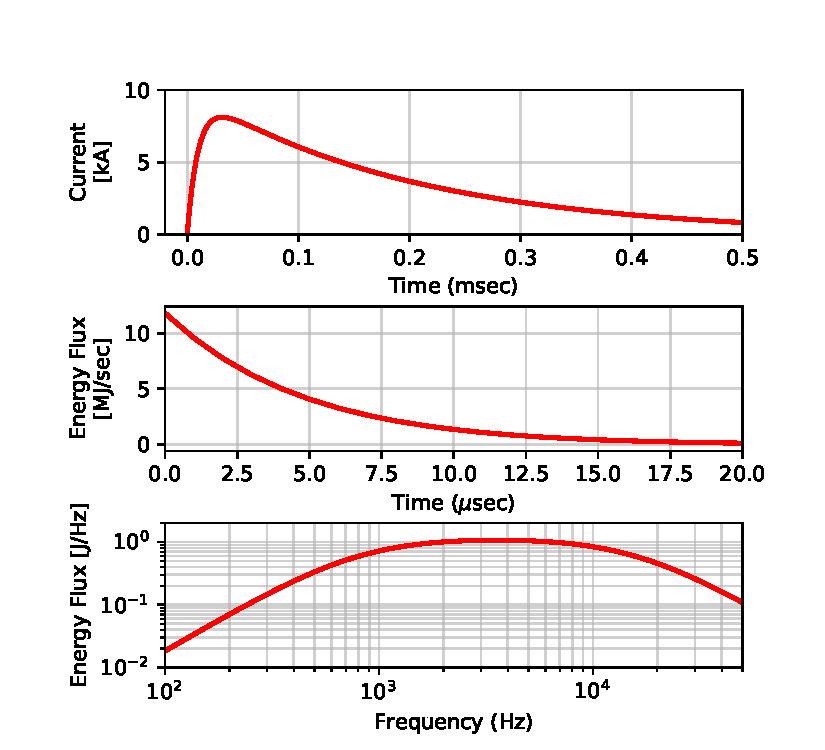
\includegraphics{figures/Lightning_spectra.pdf}

\caption{Double-exponential current pulse model of a lightning stroke. The top panel shows the stroke current vs time; the middle panel shows the total energy flux, integrated over space, vs time; the bottom panel shows the energy flux in the frequency domain.}
\label{fig:lightning_spectrum}
\end{center}
\end{figure}

\subsection{Trans-Ionosphere Attenuation}

\section{Ray Tracing and Landau Damping}
\section{Wave-Particle Interactions}
\section{Environment Models}
\subsection{Magnetic Field}
\subsection{Ionosphere}
\subsection{Plasmasphere}
The plasmasphere is a region of the space environment surrounding the Earth, and a primary unknown within our modeling. The plasmasphere extends from an altitude of ~1000km up to several Earth radii; typically it is divided into two separate regions: a dense, relatively cold \emph{inner plasmasphere}, and a sparse, relatively hot \emph{outer plasmasphere} or \emph{trough}. The transition boundary between the two regions is a sharp dropoff in plasma density called the \emph{plasmapause}.

Much like the ionosphere, the plasmasphere is a highly variable region, depending on solar conditions ($K_p$), location (latitude, longitude, field line), and time of day (MLT). The large spatial scales, high variability, and sparse availability of in-situ measurements require us to turn to empirical models of each region. We consider three primary models of electron density, and two of electron temperature.

\subsubsection{Overview of Plasmasphere Density Models}

\paragraph{Ngo Model}

The Ngo model is a legacy model used extensively in research at Stanford from the early 1980s through the mid-2000s, notably by \cite{Lauben1998} and \cite{Bortnik2005}. The model uses a Diffusive Equilibrium (DE) model for the inner and outer plasmasphere, onto which the \cite{Carpenter1992} inner plasmasphere model is overlaid. This model was integrated into the legacy Stanford VLF raytracing code, and provided several adjustable parameters, including plasmapause location, constituent ratios, and the ability to include ducts.

\paragraph{Global Core Plasmasphere Model}

The Global Core Plasmasphere Model (GCPM), initially developed in 2000 by \cite{Gallagher1999} with significant updates through the following decade, smoothly transitions between several regional models to provide a continuous model of the plasmasphere. Within this work we use version 2.4, which was released in 2009 and made available by the . GCPM incorporates the \cite{Carpenter1992} inner plasmasphere model and the \cite{Gallagher1995} outer plasmasphere model, with an empirical fit of the plasmapause location between. The polar cap model is derived from \cite{Persoon1983} and \cite{Chandler1991}. All models are connected smoothly to the IRI model of the ionosphere at lower altitudes. The combined GCPM model is parameterized by $K_p$ and MLT.

\paragraph{Simplified GCPM}

GCPM aims to provide a dynamic, complete picture of the plasmasphere as a function of time and $K_p$; however for our purposes GCPM provides too much variation. Additionally, the combination and smoothing between many models is computationally slow. In order to provide quicker computation and to reduce the number of parameters to adjust, we have implemented a simplified version of GCPM.

This model uses the equatorial-plane GCPM model, including the plasmapause location. However we omit any variation along latitude, and assume densities are constant along each field line. As our region of interest lies primarily within low and mid latitudes, we omit the polar cap model altogether and simply merge the ionosphere into the equatorial trough model. Finally to simplify computation, we model the ionosphere using an empirical fit to IRI -- one for noon, and one for midnight, with a smooth transition along longitude.

Figure \ref{fig:plasma_model_comparison} shows a side-by-side comparison of the three models.
\begin{figure}[h]
\begin{center}
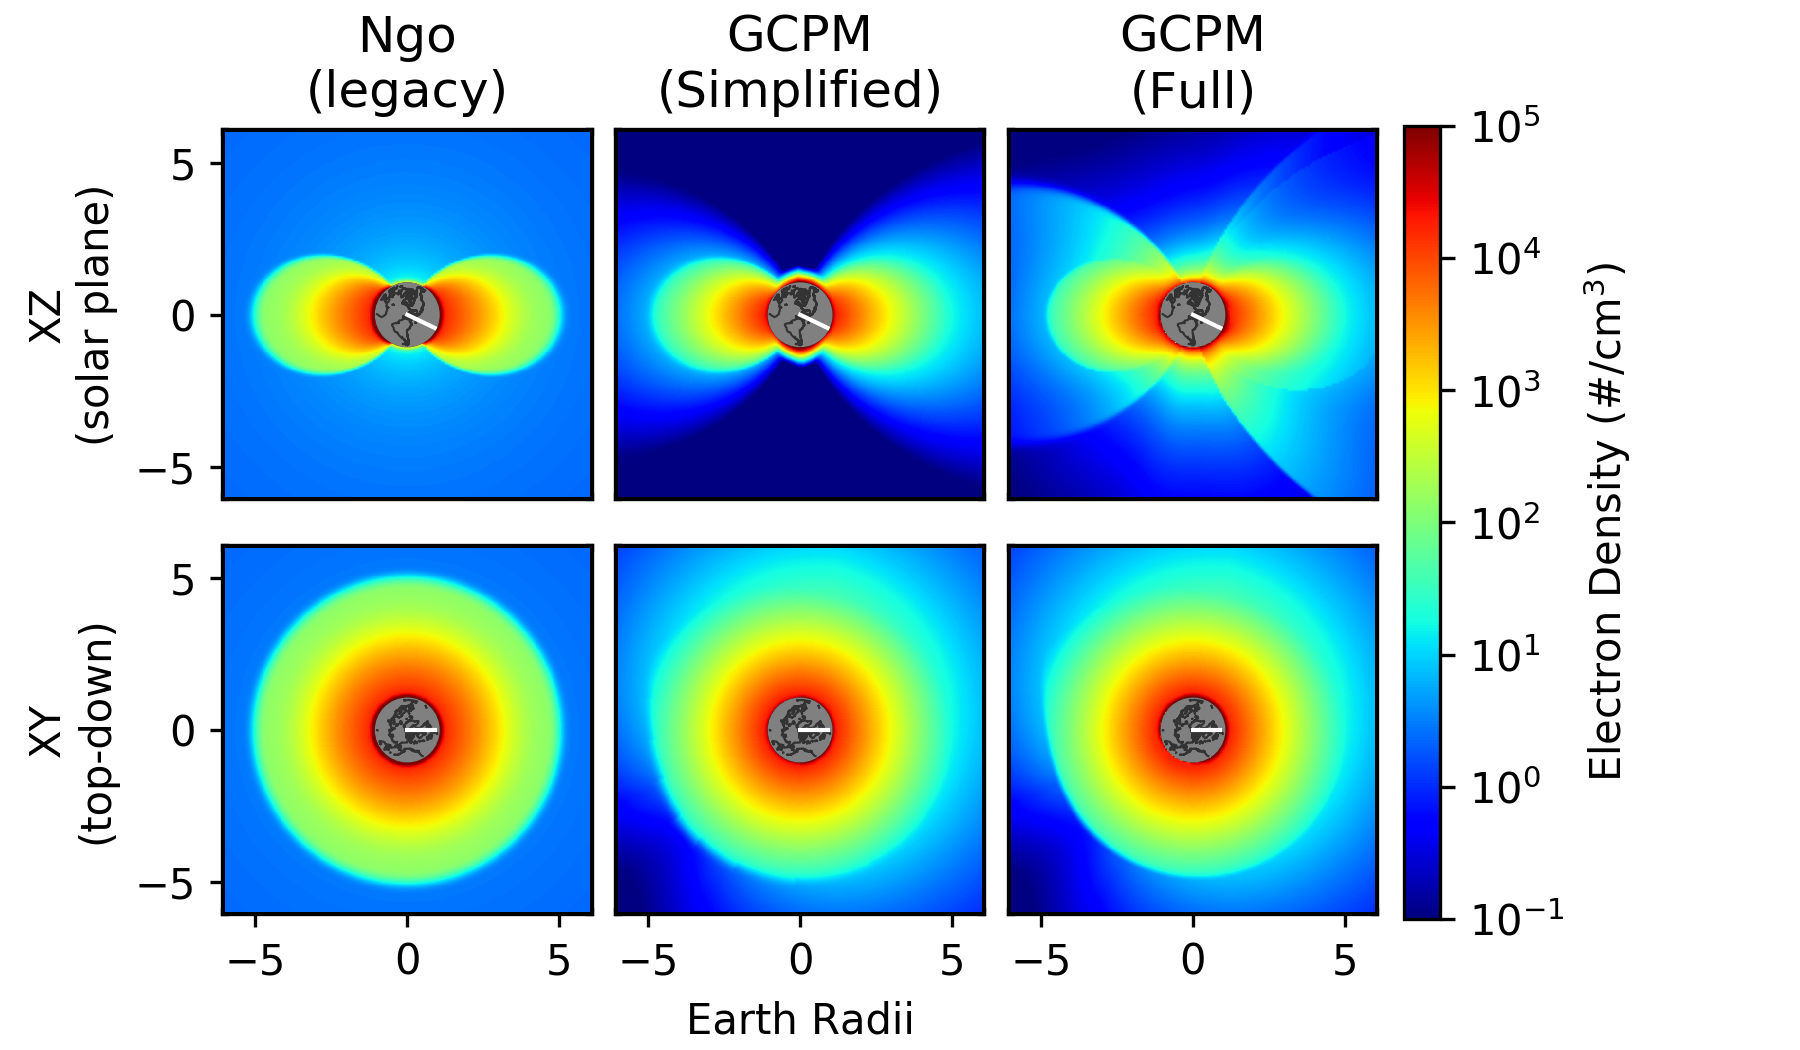
\includegraphics{figures/plasma_model_comparison.png}
\caption{A comparison of three plasmasphere models: Ngo, simplified GCPM, and full GCPM, for a relatively quiet plasmasphere ($K_p=2$). The top row shows electron density in-plane with the direction of solar influx; the bottom row shows a top down (equatorial cross-section) view. The white line indicates the solar axis. Only electron density is shown, as additional plasma constituents are derived from electron density.}
\label{fig:plasma_model_comparison}
\end{center}
\end{figure}